% -*- coding: utf-8 -*-
% vim: autoindent expandtab tabstop=4 sw=4 sts=4 filetype=tex
% vim: spelllang=de spell
% chktex-file 27 - disable warning about missing include files

\section{Sequenz-Diagramme}
\label{sec:sequence-diagrams}

Gemäss~\cite{larman_applying_2004} stellen Sequenz-Diagramme Ereignisse, welche
externe Akteure auslösen bzw.\ generieren, deren Ablauf sowie Ereignisse
zwischen Systemen eines spezifischen Szenarios eines Use Cases dar.

Da Sequenz-Diagramme schnell eine gewisse Grösse und auch Komplexität annehmen
wird in dieser Projektarbeit darauf verzichtet ein Sequenz-Diagramm für alle
Use Cases zu erstellen. Gerade bei ``UC2: Erstellen einer Echtzeit-Animation''
würde dies ansonsten grosse Ausmasse annehmen. Bei Bedarf können diese bei den
einzelnen Iterationen bzw.\ Phasen (Elaboration, Construction und Transition)
der darauffolgenden Projektarbeit noch erarbeitet werden. An dieser Stelle wird
daher nur das Sequenz-Diagramm für den ersten Use Case, ``UC1: Betrachten einer
Echtzeit-Animation'' dargestellt. Dies deckt bereits einen Teil des Editors mit
ab.

Das Sequenz-Diagramm in~\autoref{fig:sequence-diagrams:uc1} stellt das Erfolgsszenario
dar. Die Erweiterungen werden bewusst nicht dargestellt.\\
Nachfolgend wird der Ablauf des Erfolgsszenarios beschrieben.

\begin{enumerate}
    \item{%
            Der Betrachter startet die Player-Applikation. Voraussetzung ist hierbei ein
            gültiges Demoskript mitsamt den benötigen Ressourcen der exportieren
            Echtzeit-Animation. Idealerweise beinhaltet ein Export nur zwei Dateien: Die
            Player-Applikation sowie eine binär beziehungsweise eine komprimierte Datei mit
            dem Demoskript und allen benötigten Ressourcen.
        }

    \item{%
            Der Player öffnet einen Setup-Dialog, mittels welchem der Betrachter die
            gewünschte Auflösung sowie Bit-Tiefe wählt.\\
            Der Player entpackt und lädt dann das Demoskript. Darauffolgend wird die Engine
            und die Grafik-Schnittstelle (und somit auch das Hauptfenster des Players)
            initialisiert. Danach importiert der Player das Demoskript.
        }

    \item{%
            Ausgehend von diesem findet er den Hauptknoten des Graphen, DemoNode. Auf
            diesem, beziehungsweise auf dessen Interface oder Hauptklasse --- Node --- ruft
            er dann die Process-Methode zum Zeitpunkt 0 auf. Dies hat zur Folge, dass der
            komplette Szenegraph aufgebaut und (vor-) evaluiert wird. Details dieses
            Schrittes respektive dieser Schritte sind im Sequenz-Diagramm mittels gelben
            Notizen annotiert.
        }

    \item{%
            Der Player startet darauf den Timer um die Zeit messen zu können. Darauffolgend
            wird die Haupt-Schleife des Players gestartet. Es handelt sich dabei um eine
            While-Schleife, welche als Abbruchbedingung entweder den Input des Betrachters
            (in Form der Escape-Taste beispielsweise) oder keine gültige Sequenz mehr hat.
        }

    \item{%
            In der Haupt-Schleife wird jeweils der aktuelle Zeit-Stempel geholt und danach
            wird di\textsc{}eser als Argument für die Process-Methode des Hauptknotens des Graphen
            verwendet. Diese ist nicht nochmal im Detail aufgeführt, da der Ablauf derselbe
            wie beim vorherigen Aufruf ist. Schliesslich wird das berechnet Bild zum
            aktuellen Zeitpunkt mittels Renderer dargestellt.
        }

    \item{%
            Bricht der Betrachter die Haupt-Schleife mittels Taste ab oder ist keine
            gültige Sequenz mehr vorhanden, beendet sich der Player.
        }
\end{enumerate}

\begin{figure}[H]
    \centering
    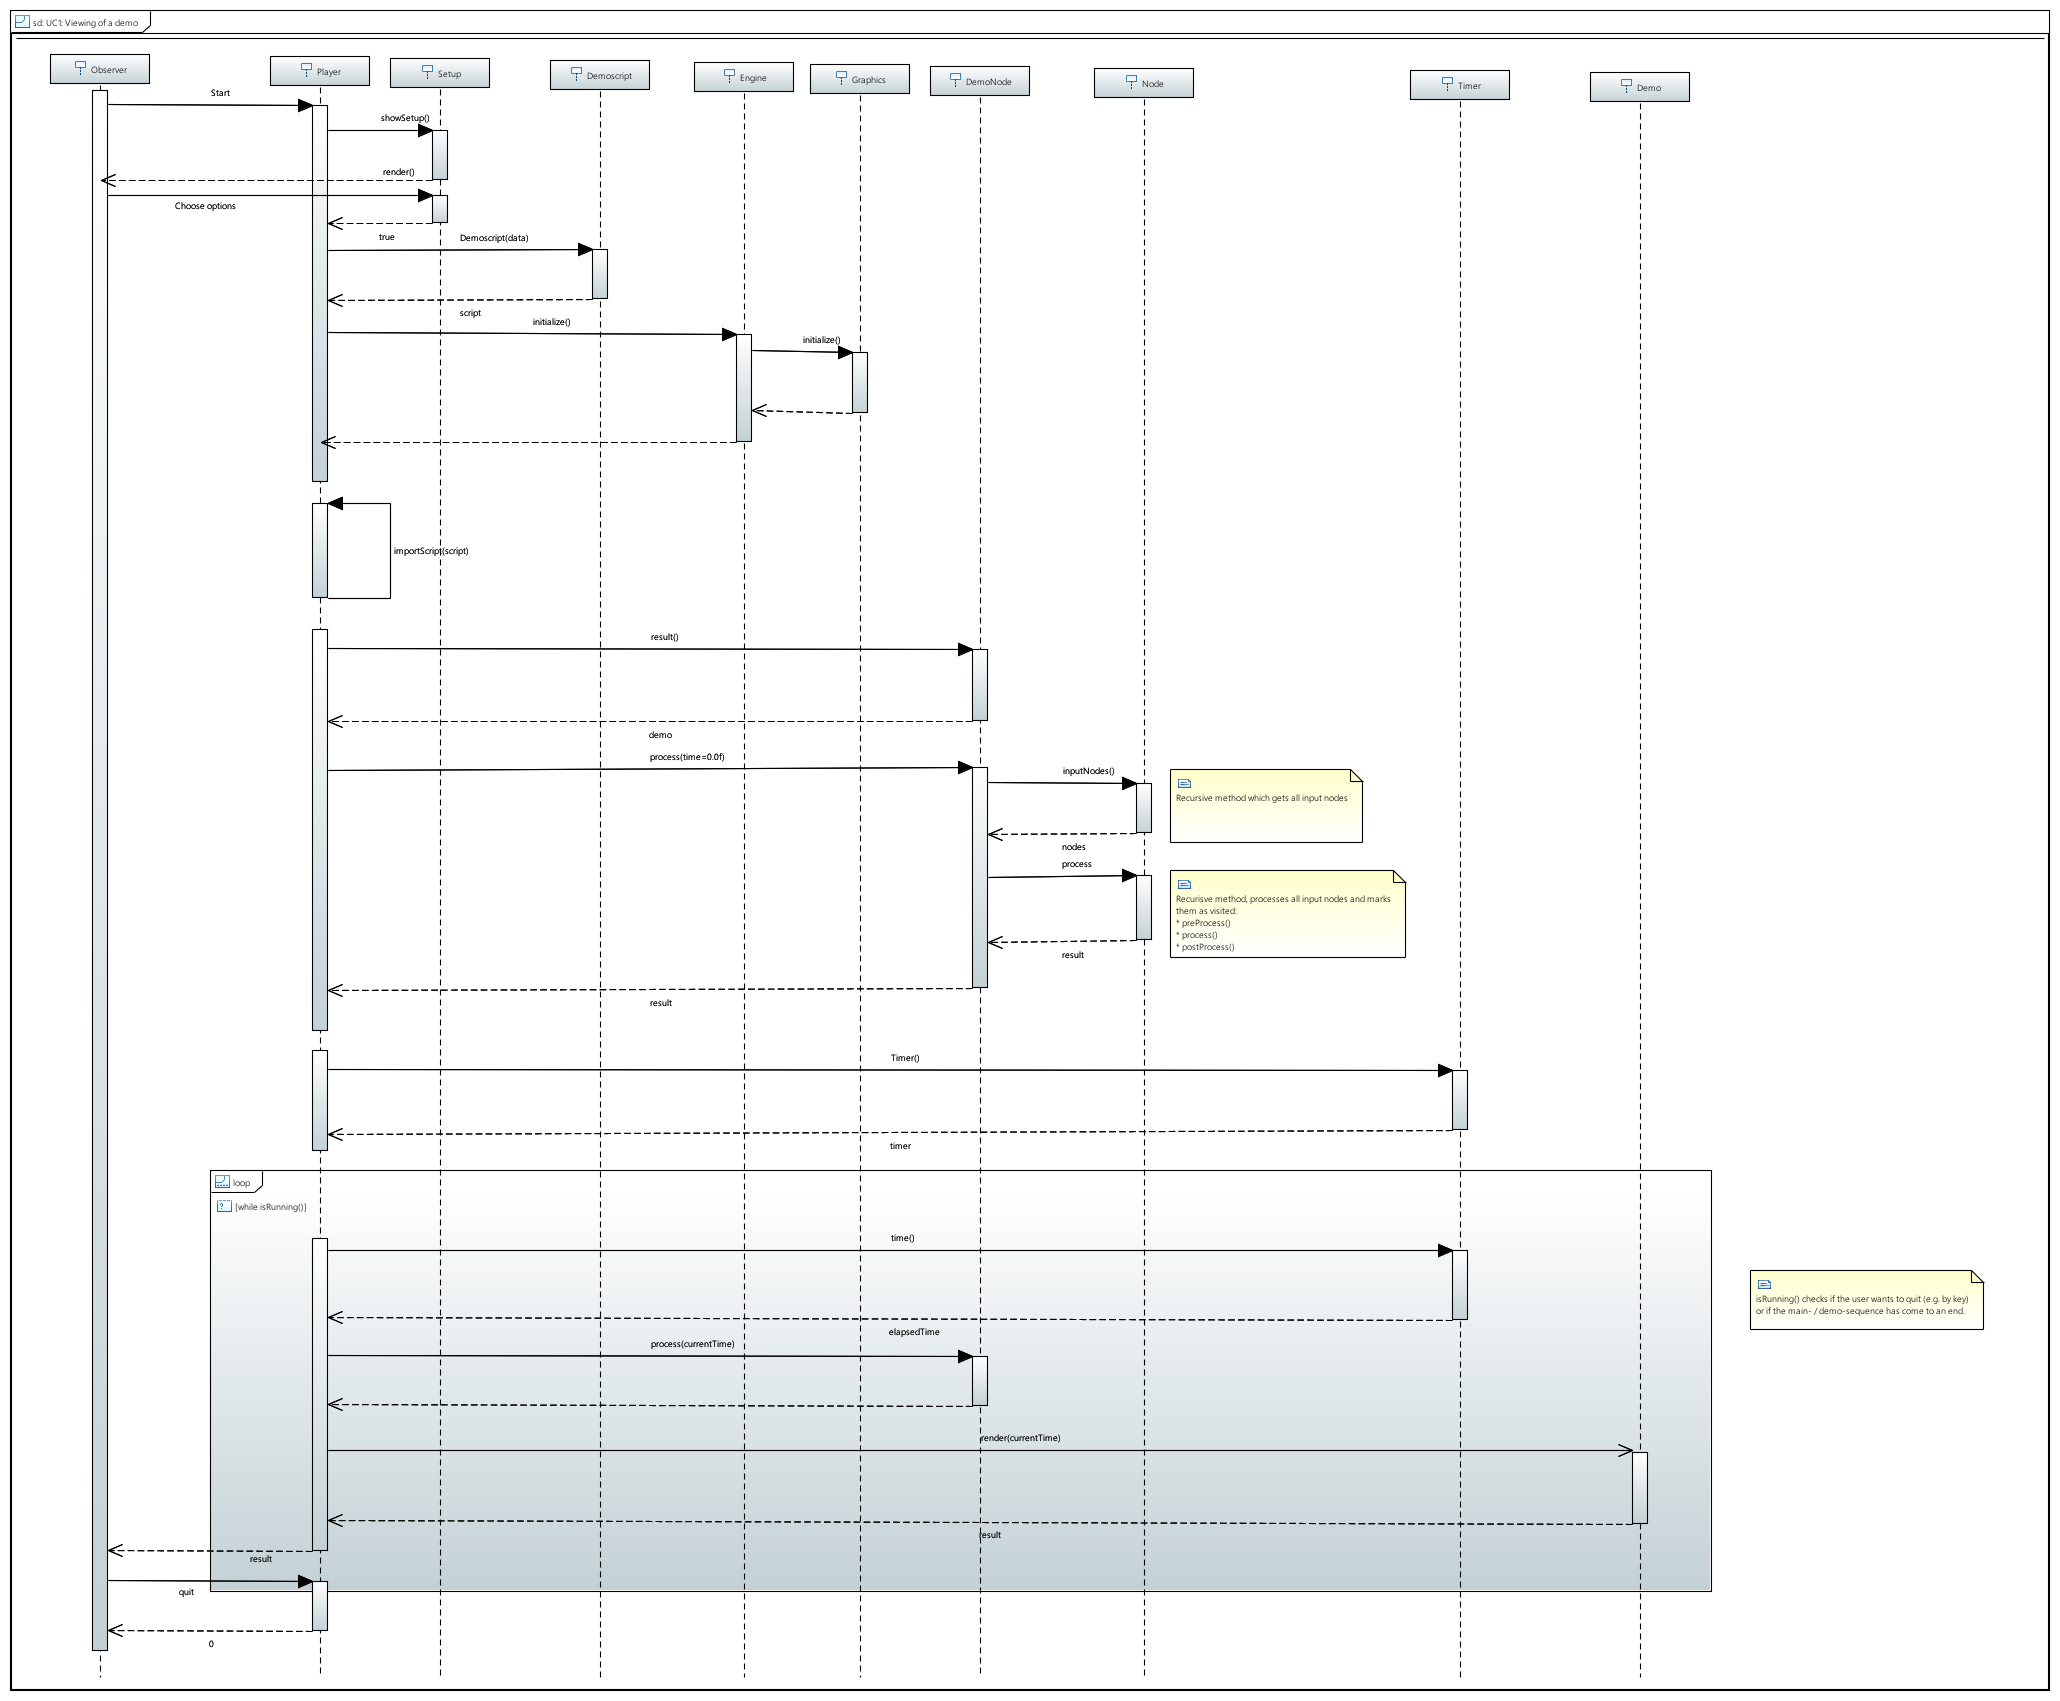
\includegraphics[angle=90,width=1.0\textwidth]{img/sequence_diagram_uc1.PNG}
    \caption{Sequenz-Diagramm des Use Cases
        UC1}\label{fig:sequence-diagrams:uc1}
\end{figure}
